% \begin{figure}[ht!]
%\begin{center}
\documentclass [tikz] {standalone}

%common figure styles
\input{header.htex}


\begin {document}

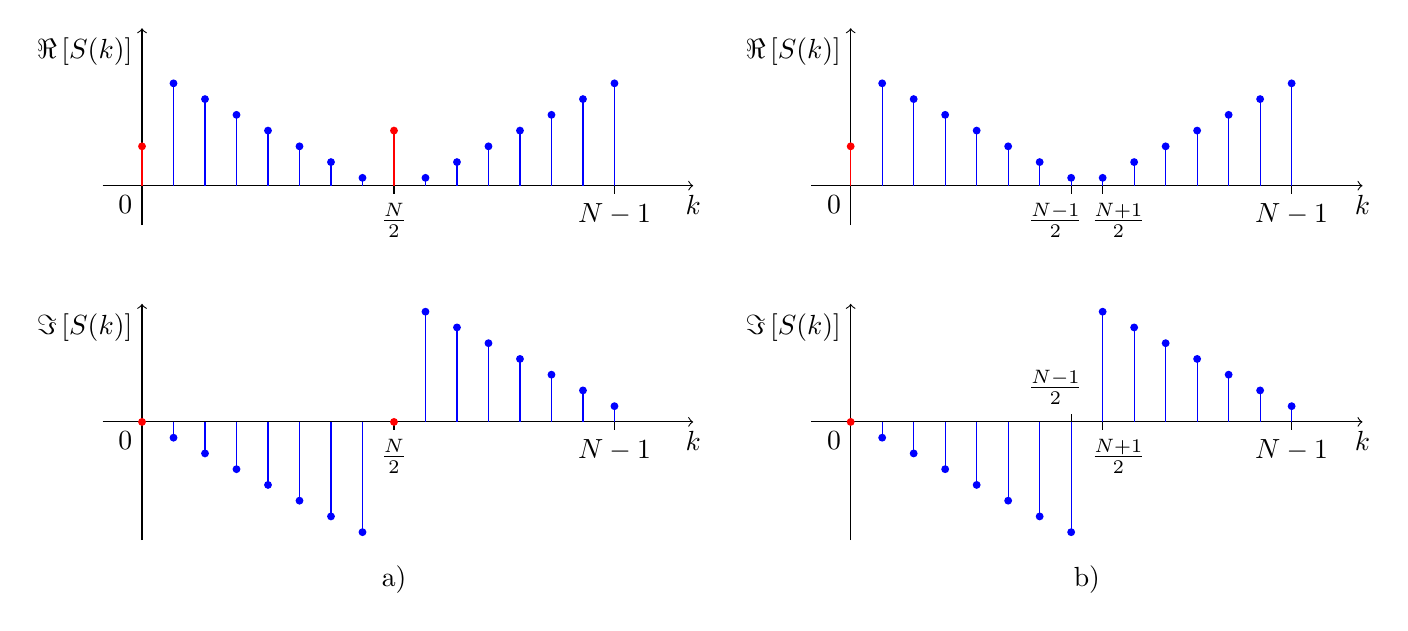
\begin{tikzpicture}



\draw[->] (-0.5, 0) -- (7, 0) node[below]{$k$};
\draw[->] (0, -0.5) -- (0, 2) node[below left]{$\Re\left[ S(k)\right]$};


\draw[->] (-0.5, -3) -- (7, -3) node[below]{$k$};
\draw[->] (0, -4.5) -- (0, -1.5) node[below left]{$\Im\left[ S(k)\right]$};







\draw[->] (8.5, 0) -- (15.5, 0) node[below]{$k$};
\draw[->] (9, -0.5) -- (9, 2) node[below left]{$\Re\left[ S(k)\right]$};


\draw[->] (8.5, -3) -- (15.5, -3) node[below]{$k$};
\draw[->] (9, -4.5) -- (9, -1.5) node[below left]{$\Im\left[ S(k)\right]$};





\draw (3.2,-5) node {a)};
\draw (12, -5) node {b)};




\draw (0,0) node[below left] {$0$};
\draw (9,0) node[below left] {$0$};
\draw (0,-3) node[below left] {$0$};
\draw (9,-3) node[below left] {$0$};


\draw[thin] (3.2, 0)  -- (3.2, -0.1) node[below] {$\frac{N}{2}$};
\draw[thin] (3.2, -3) -- (3.2, -3.1) node[below] {$\frac{N}{2}$};


\draw[thin] (6, 0)  -- (6, -0.1) node[below] {$N-1$};
\draw[thin] (6, -3) -- (6, -3.1) node[below] {$N-1$};


\draw[thin] (14.6, 0)  -- (14.6, -0.1) node[below] {$N-1$};
\draw[thin] (14.6, -3) -- (14.6, -3.1) node[below] {$N-1$};


\draw[thin] (11.8, 0)  -- (11.8, -0.1) node[below, xshift=-0.2cm ] {$\frac{N-1}{2}$};
\draw[thin] (12.2, 0)  -- (12.2, -0.1) node[below, xshift= 0.2cm ] {$\frac{N+1}{2}$};


\draw[thin] (11.8, -3)  -- (11.8, -2.9) node[above, xshift=-0.2cm] {$\frac{N-1}{2}$};
\draw[thin] (12.2, -3)  -- (12.2, -3.1) node[below, xshift= 0.2cm] {$\frac{N+1}{2}$};



\draw[red]  (0, 0)  -- (0, 0.5);
\fill[red] (0, 0.5) circle(0.05cm);


\draw[red] (3.2, 0) -- (3.2, 0.7);
\fill[red] (3.2, 0.7) circle(0.05cm);

\draw[red] (9, 0) -- (9, 0.5);
\fill[red] (9, 0.5) circle(0.05cm);



\fill[red] (0, -3) circle(0.05cm);


\fill[red] (3.2, -3) circle(0.05cm);

\fill[red] (9, -3) circle(0.05cm);




\foreach \z in {1, 2, ..., 7}
{
	
	\draw [blue] (\z *0.4, - 0cm) -- (\z*0.4, 1.5 - \z*0.2 );
	\fill [blue] (\z*0.4, 1.5 - \z*0.2 ) circle(0.05cm);
	
	\draw [blue] (\z *0.4 + 3.2, - 0cm) -- (\z*0.4 + 3.2, \z*0.2 -0.1 );
	\fill[blue] (\z*0.4+ 3.2, \z*0.2 -0.1 ) circle(0.05cm);
	
	
	
	
	
	\draw [blue] (\z *0.4, -3) -- (\z*0.4, -3 - \z*0.2 );
	\fill [blue] (\z*0.4, -3 - \z*0.2 ) circle(0.05cm);
	
	\draw [blue] (\z *0.4 + 3.2, -3) -- (\z*0.4 + 3.2, -3 -\z*0.2 +1.6 );
	\fill[blue] (\z*0.4 + 3.2, -3 -\z*0.2 +1.6) circle(0.05cm);
	
	
	
	
	
	\draw [blue] (9+\z *0.4, - 0cm) -- (9+ \z*0.4, 1.5 - \z*0.2 );
	\fill [blue] (9+\z*0.4, 1.5 - \z*0.2 ) circle(0.05cm);
	
	\draw [blue] (9+\z *0.4 + 2.8, - 0cm) -- (9+\z*0.4 + 2.8, \z*0.2 -0.1 );
	\fill [blue] (9+\z*0.4+ 2.8, \z*0.2 -0.1 ) circle(0.05cm);
	
	
	
	
	
	\draw [blue] (9+\z *0.4, -3) -- (9+\z*0.4, -3 - \z*0.2 );
	\fill [blue] (9+\z*0.4, -3 - \z*0.2 ) circle(0.05cm);
	
	\draw [blue] (9+\z *0.4 +2.8, -3) -- (9+\z*0.4 + 2.8, -3 -\z*0.2 +1.6 );
	
	\fill[blue] (9+\z*0.4 + 2.8, -3 -\z*0.2 +1.6) circle(0.05cm);
	

	
}
	      		



\end{tikzpicture}
\end {document}
  
